\chapter{Начало разработки}

\section{Развитие генераторов сигналов}
История развития генераторов сигналов начинается с аналоговых устройств, которые
использовались для генерации различных форм сигналов, включая низкочастотные,
высокочастотные, сверхвысокочастотные и импульсные. <<Во времена СССР потребности в новых средствах генерации сигналов удовлетворялись разработкой огромного числа всевозможных аналоговых генераторов сигналов>>~\cite{dgs}. Однако, с развитием технологий и потребностями в более сложных и модулируемых сигналах, стало очевидно необходимость в универсальных генераторах сигналов, способных генерировать сигналы типовых форм, такие как синусоидальные, прямоугольные, пилообразные и треугольные.

В результате развития технологий и потребностей в более сложных и модулируемых
сигналах, появились новейшие разработки генераторов сигналов на основе прямого
цифрового синтеза частот и форм сигналов. Эти генераторы сигналов используют минимальное количество аналоговой элементной базы и основываются на стандартных и
специализированных сверхскоростных цифровых микросхемах, а также аналого-цифровых (АЦП) и цифро-аналоговых (ЦАП) преобразователях. Это позволяет легко интегрировать такие генераторы с цифровыми системами и современными компьютерами, открывая широкие возможности их применения в испытании и отладке различных электронных и радиотехнических систем и устройств. 

В современной измерительной технике генераторы сигналов играют ключевую роль, особенно в области электронно-оптических приборов, видеоимпульсных и ультразвуковых локаторов, гео- и подповерхностных радаров, а также в системах цифровой связи, включая мобильные системы. Несмотря на то, что в прошлом развитие в этой области было активно, в настоящее время наблюдается отставание от многих передовых направлений применения электронных устройств, включая микропроцессоры, работающие на частотах в единицы ГГц и выше. 

Важно отметить, что развитие генераторов сигналов тесно связано с развитием полупроводниковой технологии  элементной базы. В частности, были проведены значительные исследования в области германиевых и кремниевых транзисторов в лавинном режиме работы, что позволило разработать уникальные импульсные устройства и генераторы мощных импульсов. Однако, после распада СССР, многие из этих разработок были прерваны, и на рынок начали поступать зарубежные разработки. В целом, история развития генераторов сигналов отражает эволюцию технологий, потребностей в модулируемых сигналах и влияние глобальных изменений в науке и технике.


\section{Обзор существующих генераторов на рынке}
Сейчас на рынке присутствуют несколько видов генераторов:
\begin{enumerate}
	\item Генераторы синусоидальных сигнал.
	\item Генераторы импульсов.
	\item Функциональные генераторы.
	\item Генераторы сигналов произвольной формы.
\end{enumerate}

\subsection{Генераторы синусоидальных сигналов}
Генераторы таких сигналов широко применяются при тестировании различных радиоэлектронных устройств. <<Достоинством обычных генераторов синусоидальных сигналов является возможность получения синусоидальной формы выходного сигнала с малыми нелинейными искажениями. А главным недостатком — низкая стабильность частоты.>>~\cite{dgs}. 

\subsection{Генераторы импульсов}
Генерация импульсов необходима для тестирования и отладки импульсных систем. Это может быть радиолокатор или устройства и цифровые системы различного назначения. Такого рода генераторы находят большое применение в качестве источников несинусоидальных сигналов.

\subsection{Функциональные генераторы}
Данные устройства генерируют сигналы разной формы. Их простота и плавная регулировка частоты в большом диапазоне привела к массовому применению генераторов такого типа.

\subsection{Генераторы сигналов произвольной формы}
Достаточно новое направление в генераторах сигналов, которое основывается на прямом цифровом синтезе различных сигналов, по сути произвольных форм.

\section{Методы программной генерации сигнала}
	Основные методы цифровой генерации сигналов --- метод аппроксимации и табличный метод.
	
	Метод аппроксимации подразумевает собой вычисление отсчётов функции с заданным интервалом. В памяти хранятся только параметры сигнала. Поэтому данный метод позволяет затратить небольшой объём памяти, но его недостаток это затраты на вычисления, что ограничивает максимальную частоту сигнала.
	
	В табличном методе генерации сигналов предполагается, что заранее вычисленные отсчёты хранятся в памяти. То есть никаких вычислений не требуется и генерация сводится к тому, что в порт цифро-аналогового преобразователя нужно вывести ячейку по заданному адресу. Таким образом, время на формирование отсчёта становится меньше и появляется возможность генерировать сигнал с более высокой частотой. Недостатком же является большие затраты памяти.
	
	Будем рассматривать табличный метод синтеза. Для начала потребуется таблица отсчётов, чтобы её вычислить используем готовый инструмент.
	
	\begin{figure}[H]
    \centering
    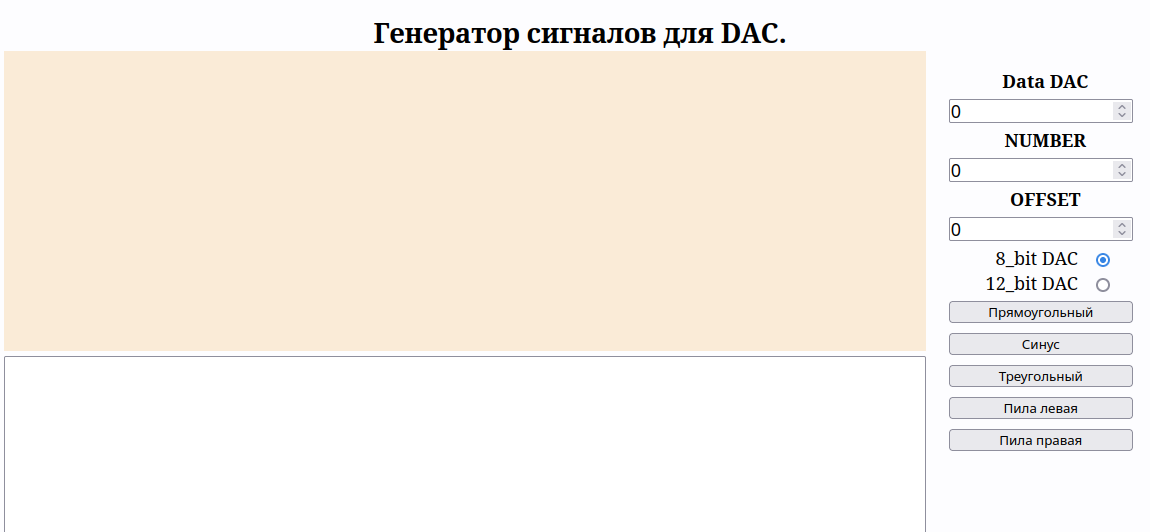
\includegraphics[width=1\textwidth]{../image/lut_prog.png}
    \caption{Программа для вычисления значений сигнала.}
	\end{figure}
	
	У таблицы есть 4 параметра:
	\begin{enumerate}
		\item Разрядность ЦАП: 8 или 12 бит.
		\item Максимальное значение.
		\item Количество значений.
		\item Смещение от нуля.
	\end{enumerate}
	
	Использовать мы будем 12-битные значения в количестве 256 чисел. Максимальное значение амплитуды сигнала может быть 4095, но так как для улучшения генерации будет задействован встроенный в цифро-аналоговый преобразователь выходной буфер, то он будет срезать сигнал сверху и снизу на 0.2В, поэтому значения тоже следует срезать на эту же величину для корректной генерации.
	
	В документе от ST про работу с цифро-аналоговым преобразователем есть формула для расчета выходного напряжения.
	
	$DAC_{output} = V_{REF}*\dfrac{DOR}{DAC_{MaxDigitalValue} + 1}$, где DOR --- цифровое значение.
	
	Нам нужно найти какое значение соответствует напряжению 0.2В. Выразим DOR и подставим имеющиеся значения.
	
	$DOR = \dfrac{V_{REF}}{DOR}*DAC_{MaxDigitalValue} + 1 = \dfrac{3.3}{0.2}*(4095+1) = 248$
	
	Укажем смещение от нуля 248, а максимальное значение 4095 меньше на 248, то есть 3847 и сгенеририуем таблицу отсчётов для синусоиды. 
	
	\begin{figure}[H]
    \centering
    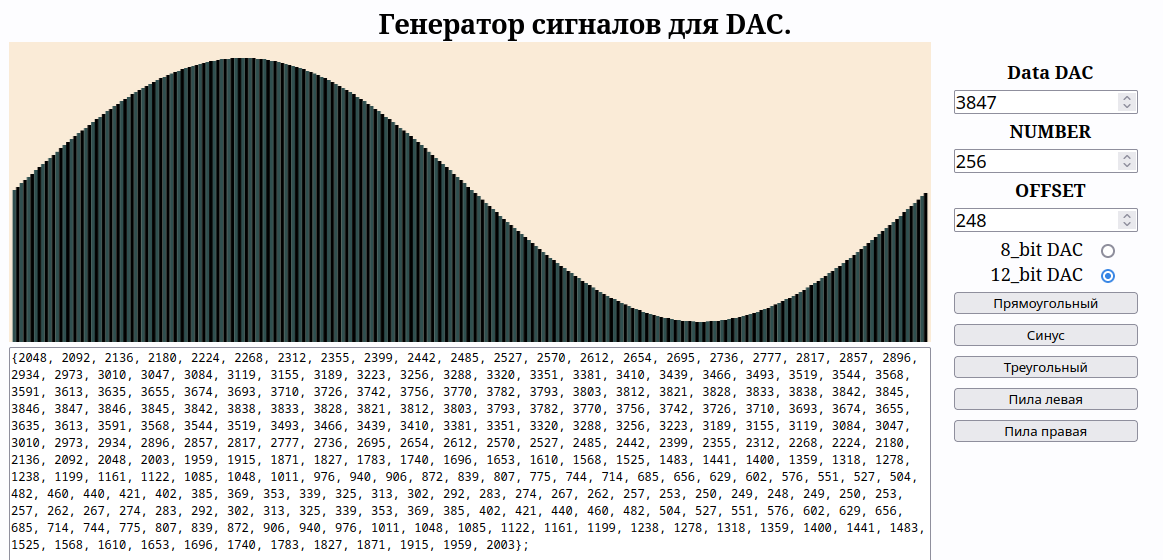
\includegraphics[width=1\textwidth]{../image/lut.png}
    \caption{Вычисление таблицы сигнала.}
	\end{figure}
	
	Теперь у нас есть данные для генерации сигнала, но теперь нужно продумать как передавать их в цап и как вообще работать с цапом.
	
	